% -*- root: Main.tex -*-

\section{SVMs and Lagrange Multipliers}

\subsection*{Lagrange Multipliers}
find $w^* = \text{argmin}_w f(w)$ s.t. $g(w)=0$, $h(w) \leq 0$\\
$\Rightarrow \nabla f(w^*) + \lambda \nabla g(w^*) + \alpha \nabla h(w^*) = 0$ with \\ complete slackness $a \geq 0$, $\alpha h(w^*)=0$ \\
\textbf{conv. optimization}: 1. compute Lagrangian $\mathcal{L}(w,\lambda,\alpha)$, 2. check Slater's condition: $\exists w : g_i(w)=0$, $h_j(w) < 0$, 3. solve $\nabla_w \mathcal{L} = 0$, $g_i(w)=0$, $\alpha_j h_j (w) = 0$ with $a_j \geq 0$, $h_j(w) \leq 0$

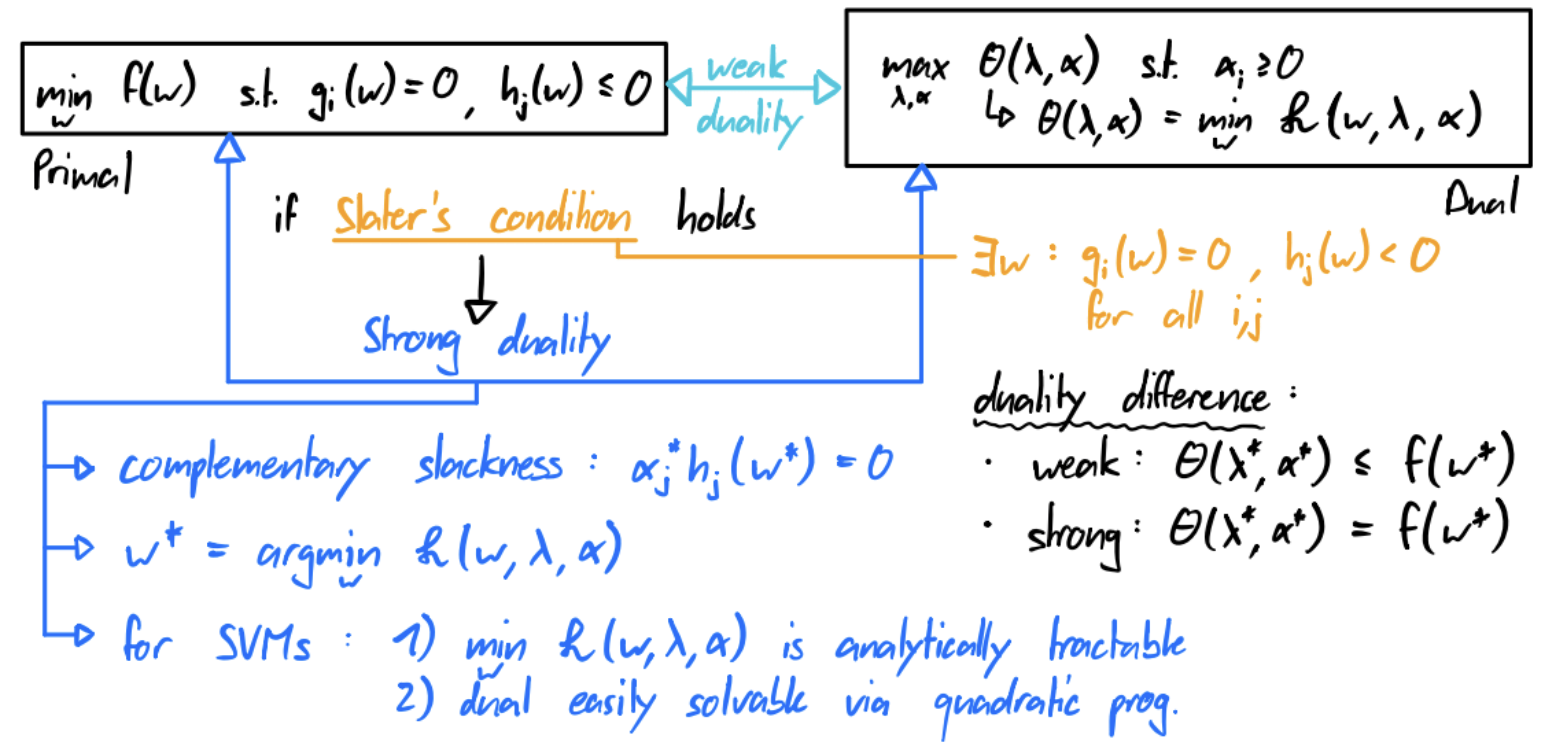
\includegraphics[width=7cm]{lagrangian multipliers.png}

\subsection*{SVMs}
\textbf{Primal Problem}: 
    {\scriptsize ($C \rightarrow \infty$: Hard Margin)}\\
    {\footnotesize $\min_w \frac{1}{2} w^Tw + C \sum_{i=1}^n \xi_i$ s.t. $y_i(w^T x_i +w_0) \geq 1-\xi_i, \, \xi_i \geq 0$ }\\
\textbf{Dual Problem}:
    $\mathcal{L}(w, w_0, \lambda, \alpha) = \frac{1}{2} w^\top w + \sum_{i \leq n} \alpha_i (1 - y_i(w^\top x_i + w_0))$, $\alpha_i \geq 0$ \\
    {\footnotesize $\Rightarrow \mathcal{L}(w^*, w_0^*, \lambda, \alpha) = - \frac{1}{2} \sum_{i,j} \alpha_i \alpha_j y_i y_j x_i^\top x_j + \sum_i \alpha_i$} \\
    $\Rightarrow \max_\alpha \alpha_i - \frac{1}{2} \sum_{i,j} \alpha_i \alpha_j \y_i y_j x_i^\top x_j$ s.t $\alpha_i \geq 0$, $\sum_i \alpha_i y_i = 0$ \\
    	%$\mathcal{L}(w,w_0,\xi,\alpha,\beta) = \frac{1}{2}w^Tw + C\sum_{i=1}^n\xi_i - \sum_{i=1}^{n}\beta_i\xi_i \\
        %\tab\tab\tab-\sum_{i=1}^{n} \alpha_i(z_i(w^T\phi(y_i) + w_0) -1+\xi_i)\\
		%\max_\alpha L(a) = \sum_{i=1}^n\alpha_i - \frac{1}{2} \sum_{i,j=1}^n z_i z_j 
		%\alpha_i \alpha_j \phi(y_i, y_j)\\
		%s.t. \, \sum_{j=1}^n z_j \alpha_j = 0 \, \wedge C \geq \alpha_i \geq 0 $\\
    $\Rightarrow$ optimal hyperplane:  $w^* = \sum_{i=1}^n \alpha_i^* y_i \phi(x_i)$, \\
    $w_0^* = -\frac{1}{2} (w^*^\top x^+ + w^*^\top x^-$ 
%    $w_0^* = \frac{1}{n_s} \sum_{i \in S}(z_n - \sum_{j \in S} \alpha_j z_j \phi(y_i,y_j))\\
%    		\stackrel{\text{\tiny linear}}{=} -\frac{1}{2}(min_{i:z_i=1} w^{*T}y_i + max_{i:z_i=-1} w^{*T}y_i)$\\
%Only for support vectors:\mbox{} $\alpha_i^* > 0$\\
%Prediction:\mbox{} 
%	$z(y)=sign(\sum_{i=1}^n \alpha_i z_i \phi(y,y_i) + w_0) \\
%        \stackrel{\text{\tiny linear}}{=} sign(w^{*T}x+w_0)$\\
%Homog. Coordinates:\mbox{}  condition $\sum_{j=1}^n z_j \alpha_j = 0$ falls away.

\subsection*{Kernelized SVMs}
\textbf{Training}: $\min_{\alpha} \sum_{i\leqn} \alpha_i - \frac{1}{2} \sum_{i,j \leq n} \alpha_i \alpha_j y_i y_j k(x_i, x_j)$ s.t. $\alpha \geq 0$, $\sum_i \alpha_i y_i = 0$ \\
\textbf{Classify}: $y = sign(\sum_{i \leq n} \alpha_i y_i k(x_i, x))$

\subsection*{Multiclass SVMs}
$\min_{w, \xi\geq 0} \frac{1}{2} w^T w + C \sum_i \xi_i$ s.t. \\
$(w_{y_i}^\top x_i + w_{y_i, 0}) - \max_{y \neq y_i} (w_y^\top x_i + w_{y,0}) \geq 1 - \xi_i$
%s.t. $\forall y_i \in Y:( w_{z_i}^T y_i) - max_{z \not = z_i} (w_z^T y_i) \geq 1-\xi_i$

\subsection*{Structured SVMs}
$\min_{w, \xi} \frac{1}{2} w^\top w + C \sum_i \xi$ s.t. \\
$w^\top \psi(x_i, y_i) - \max_{y \neq y_i} (w^\top \psi(x_i, y) \geq 1 - \xi$

% \subsection*{How to find $a^T$?}
% $a = \{w_0,w\}$ used along $\widetilde{x} = \{1,x\}$

% Gradient Descent: $a(k+1) = a(k) - \eta(k) \nabla J(a(k))$

% Newton method: 2nd order Taylor to get $\eta_{opt} = H^{-1}$ with $H=\frac{\partial^2 J}{\partial a_i \partial a_j}$

% $J$ is the cost matrix, popular choice is


% \subsection*{Perceptron Algorithm}
% Stochastic Gradient + Perceptron loss\\

% \emph{Theorem:} If $D$ is linearly seperable $\Rightarrow$ Perceptron will obtain a linear seperator.

% \subsection*{Support Vector Machine}
% Try to maximize a 'band' around the seperator.\\

% \subsection*{Matrix-Vector Gradient}
% %multiply transposed matrix to the same side as its occurance w.r.t. derivate variable: $\beta \in \mathbb{R}^d$
% $\nabla_\beta ( ||y-X\beta||_2^2 + \lambda ||\beta||_2^2 ) = 2X^T (y-X\beta) + 2\lambda \beta$\\

% \subsection*{Hinge loss}
% loss for support vector machine.\\
% $l_{SVM}(w,x_i,y_i) = \max \{0,1-y_iw^Tx_i\} + \lambda ||w||_2^2$\\
% derivation:\\
% $\frac{\partial}{\partial w_k} l_{SVM}(w,y_i,x_i) = \left \{
% \begin{array}{lr}
% 0 \text{ , if } 1-y_iw^Tx_i < 0 \\
% -y_ix_{i,k} + 2\lambda w_k \text{ , otherwise}
% \end{array} \right.	$

% \subsection*{Sparse L1-SVM}
% $\underset{w}{\operatorname{argmin}} \sum \limits_{i=1}^n \max (0, 1-y_i w^T x_i) + \lambda ||w||_1$
